\section{Formazione stellare}\linkdest{sec:cloudscollapse}

\subsection{Fase isoterma}

\begin{frame}{Collasso nube inter-stellare}
\begin{block}{Condizione di collasso}
Prima fase: collasso isotermo.
\begin{columns}
\begin{column}{0.5\textwidth}
$\TtwoDy{t}{I}<0$ quindi $E_T+U<0$.
\end{column}
\begin{column}{0.5\textwidth}
Nube di $H_2$ a $T=\SI{10}{\kelvin}$:
$\rho>\num{e-18}(\frac{M}{\msun{}})^{-2}$\si{\gram\per\cubic\cm}
\end{column}
\end{columns}
\begin{block}{Nubi giganti: addensamenti}
Turbolenza crea zone pi\'u dense: Mckee ostriker 07, Folin i 14, bertelli Motta 16.
\end{block}
\begin{block}{Rotazione}
\begin{columns}[T]
\begin{column}{0.5\textwidth}
T,M,J costanti:
\begin{align*}
&E_{th}\approx c'\\
&E_{Rot}\approx c''\rho\expy{\frac{2}{3}}\\
&U\approx c'''\rho\expy{\frac{1}{3}}\\
&\alpha=\frac{E_{th}}{U},\ \beta=\frac{E_{rot}}{U}
\end{align*}
\end{column}
\begin{column}{0.5\textwidth}
Condizione di collasso proibito: $16\alpha(\rho_0)\beta(\rho_0))>1$
\end{column}
\end{columns}
\end{block}
\end{block}
\end{frame}

\begin{wordonframe}{Collasso nube inter-stellare}\tolbf
\begin{block}{Teorema viriale:todo}\end{block}
\begin{columns}[T]
\begin{column}{0.5\textwidth}
T,M,J costanti:
\begin{align*}
&E_{th}\approx c'\\
&E_{Rot}\approx\frac{1}{2}\frac{J^2}{I}=\frac{J^2}{2}\frac{1}{\frac{2}{5}MR^2}=c''\rho\expy{\frac{2}{3}}\\
&U\approx\frac{3}{5}\frac{GM^2}{R}=c'''\rho\expy{\frac{1}{3}}
\end{align*}
\end{column}
\begin{column}{0.5\textwidth}
\begin{align*}
&f(\psi=\frac{\rho}{\rho_0})=\alpha_0\psi\expy{-\frac{1}{3}}+\beta_0\psi\expy{\frac{1}{3}}\\
&\begin{pmatrix}
&f<\frac{1}{2}: \text{collasso}\\
&f>\frac{1}{2}: \text{espansione}\\
\end{pmatrix}\\
&\alpha=\alpha_0(\rho_0)(\frac{\rho}{\rho_0})\expy{-\frac{1}{3}}\\
&\beta=\beta(\rho_0)(\frac{\rho}{\rho_0})\expy{\frac{1}{3}}
\end{align*}
\end{column}
\end{columns}
f ha minimo in $\psi_0=(\frac{\alpha_0}{\beta_0\beta_0})\expy{\frac{3}{2}}$
\end{wordonframe}

\subsection{Fase adiabatica}

\begin{frame}{Inizio fase adiabatica: aumento temperatura}
\begin{block}{Aumento cammino ottico}
\begin{columns}[T]
\begin{column}{0.5\textwidth}
Cammino ottico di un fotone minore delle dimensioni della nube: $\kappa\rho R>1$.
\end{column}
\begin{column}{0.5\textwidth}
Densit\'a che consente aumento T: $\rho_{ad}\propto M\expy{-\frac{1}{3}}?$
\end{column}
\end{columns}
\end{block}
\begin{block}{Termine collasso adiabatico ($\Delta E_T=-\Delta U$)}
Equilibrio: $E_T^{ad}+\Delta E_T=\frac{1}{2}|U+\Delta U|$: $\Delta R=-\frac{R}{2}$ e $\rho'=8\rho_{ad}$.
\end{block}
\begin{block}{Comportamento pseudo-adiabatico: $P\propto\rho\expy{\gamma}$}
\begin{columns}[T]
\begin{column}{0.5\textwidth}
\begin{align*}
&T=T_0(\frac{\rho}{\rho_{ad}})\expy{\gamma-1}\\
&P=P_0(\frac{\rho}{\rho_{ad}})\expy{\gamma}
\end{align*}
\end{column}
\begin{column}{0.5\textwidth}
$\gamma>\frac{4}{3}$: $\alpha$ diventa $>\frac{1}{2}$
\end{column}
\end{columns}
Condizione di equilibrio: $\rho_{eq}\propto M\expy{\theta}\begin{pmatrix}
\approx\num{e-10}, \gamma=\frac{5}{3}\\
\approx\num{e6}, \gamma=\frac{7}{5}
\end{pmatrix}$.
\end{block}
$T>\SI{e3}{\kelvin}$: dissociazione molecolare, ionizzazione.
Zona centrale raggiunge stato di quasi-equilibrio: lenta contrazione.
\end{frame}

\begin{wordonframe}{Fase adiabatica}
$P\propto\rho\expy{\gamma}$: corrisponde a vera adiabatica  se condizione iniziale di equilibrio o qe.

Condizione di equilibrio: $kT_0(\frac{\rho_{eq}}{\rho_{ad}})\expy{\gamma-1}=\const M\expy{\frac{2}{3}}\rho_{eq}\expy{\frac{1}{3}}$.

''Solo se la temperatura aumenta rapidamente con densit\'a \'e possibile ristabilire equilibrio.''

Ionizzazione e dissociazione rallentano aumento di T e P: accelerazione collasso.

Quando la zona interna raggiunge l'equilibrio l'esterno continua a contrarsi: rimbalzi.

\end{wordonframe}

\section{Formazione planetaria}\linkdest{sec:protoplanetary}

\subsection{Osservazioni}

\begin{frame}{Cosa deve spiegare la teoria?}

\begin{itemize}
\item Massa nube interstellari molto maggiori della massa del sistema solare
\item stelle raggruppate in ammassi
\item Sistemi doppi o multipli
\item Numerosi sistemi planetari
\end{itemize}

\begin{itemize}
\item Frammentazione: presenza di condensazioni iniziali, fissione per rotazione. (moti turbolenti, jet di materia)
\item campi magnetici e rotazione inibiscono il collasso sul piano di simmetria
\item configurazioni simmetria cilindrica: toro, disco; rottura simmetria: spirale, strutture 3-assiali.
\item Popolazione Binarie strette ha picco popolazione per masse uguali, sistemi larghi hanno masse diverse (diversi canali formazione)
\item Problema momento angolare sistema solare. Trasferimento di momento verso l'esterno: turbolenza, magnetic breaking.
\end{itemize}

\end{frame}

\begin{wordonframe}{Cosa deve spiegare la teoria?}

Come si frammenta la nube interstellare? cosa differenzia l'evoluzione dei frammenti in sistemi doppi, sistemi planetari, etc

Problema momento angolare: $J_{\odot}/\msun{}=\SI{4e15}{\squared\cm\per\second}$, $J_{J}/M_J=\SI{4e20}{\squared\cm\per\second}$.

\end{wordonframe}

\begin{wordonframe}{Fatti osservativi di cui la teoria di formazione deve tenere conto}

\begin{itemize}
\item Orbite coplanari vicino all'equatore solare
\item Distanza tra orbite pianeti maggiore aumenta con distanza
\item Comete: Nube di Oort (\SI{e4}{\astronomicalunit}) con distribuzione isotropa, Kuiper belt ($>40\si{\astronomicalunit}$) con orbite planari.
\item 6 pianeti maggiori ruotano in maniera prograda con spin inclinato di meno di \ang{30}; Venere,Urano ruotano in maniera retrogada.
\item Sistemi di satelliti. Satelliti vicini al pianeta hanno piccola eccentricit\'a e inclinazione, viceversa quelli distanti.
\item I pianeti hanno $<0.2\%$ della massa del sistema solare.
\item $98\%$ del momento angolare \'e nel moto dei pianeti gioviani; il momento angolare dei satelliti dei pianeti gioviani \'e molto minore del momento dovuto allo spin dei pianeti.
\item Composizione: i pianeti terrestri sono pi\'u densi dei pianeti gioviani.
\item Fascia di asteroidi (origine meteoriti)
\item Crateri

\end{itemize}

\end{wordonframe}

\subsection{Modello nebulare}

\begin{frame}{Evoluzione disco di accrescimento}

Osservazione: $M_{d}\approx1-10^{-3}M_*$.

Tempo di vita del disco: la formazione di pianeti ha luogo quando il disco si \'e raffreddato a sufficienza.

Sistema solare: modelli a la Sofronov.

Sistemi extra-solari: modelli al la sofronov(/Cameron)

\end{frame}

\begin{wordonframe}{Accertion disk}

Dischi troppo massicci sono instabili

Inizialmente il disco riceve pi\'u massa dall'esterno di quanta cada sulla stella, successivamente perde massa fino ad esaurirsi.

La parte interna del disco si muove verso la stella, la parte esterna verso l'esterno; il confine tra le 2 zone si sposta verso l'esterno.

Problemi modello a la Cameron: dispersione maggior parte massa del disco, differenziazione composizione chimica pianeti giganti/Sole, mancanza di pianeti terrestri e corpi minori.

\end{wordonframe}

\section{Evoluzione del campo di velocit\'a di una nube interstellare: equazione di Eulero e Navier-Stokes.}

\begin{frame}{Evoluzione del campo di velocit\'a di una distro di materia.}


\begin{block}{Equazione di Eulero}
\begin{columns}[T]
\begin{column}{0.5\textwidth}
\begin{equation*}
\PDy{t}{\vec{v}}+(\scap{v}{\nabla})\cdot\vec{v}=-\frac{1}{\rho}\nabla P+\vec{g}
\end{equation*}
Non tiene conto di effetti dissipativi: viscosit\'a, scambi di calore.
\end{column}
\begin{column}{0.5\textwidth}
\begin{align*}
&\PDof{t}(v_i\rho)=-\PDof{x_k}\Pi_{ik}+\rho g_i\\
&\Pi_{ik}=P\delta_{ik}+\rho v_iv_k
\end{align*}
\end{column}

\end{columns}

\end{block}

\begin{columns}[T]

\begin{column}{0.45\textwidth}
\begin{block}{Tensore flusso d'impulso}
\begin{equation*}
\rho\PDy{t}{v_i}=-\rho v_k\PDy{x_k}{v_i}-\PDy{x_i}{P}+\rho g_i+\PDy{x_k}{\sigma_{ik}'}
\end{equation*}
\end{block}
\end{column}

\begin{column}{0.6\textwidth}
\begin{block}{Viscous stress tensor}
\begin{align*}
\sigma'_{ik}=\eta(\PDy{x_k}{v_i}+\PDy{x_i}{v_k}-\frac{2}{3}\delta_{ik}\PDy{x_l}{v_l})+\zeta\delta_{ik}\PDy{x_l}{v_l}
\end{align*}
\end{block}
\end{column}

\end{columns}

\begin{block}{Fluido incomprimibile: equazione di Navier-Stokes}
$\vec{g}=0$
\begin{equation*}
\rho\PDy{t}{\vec{v}}=-\rho(\scap{v}{\nabla})\vec{v}-\nabla P+\eta\nabla^2\vec{v}
\end{equation*}
\end{block}

\end{frame}

\begin{wordonframe}{Equazione del moto fluido: eq Eulero Navier-Stokes}

Descrizione euleriana: $\TDy{t}{\vec{v}}=\PDy{t}{\vec{v}}+\sum_i\PDy{x_i}{\vec{v}}\TDy{t}{x_i}=\PDy{t}{\vec{v}}+(\scap{v}{\nabla})\vec{v}$.

Flusso di momento:
\begin{equation*}
\PDof{t}(v_i\rho)=\rho\PDy{t}{v_i}-v_i\PDy{x_k}{(\rho v_k)}=-\PDof{x_k}(\rho v_iv_k)-\delta_{ik}\PDy{x_k}{P}+\rho g_i=-\PDof{x_k}\Pi_{ik}+\rho g_i
\end{equation*}

Viscous stress tensor: Nullo per moto uniforme; nullo per rotazione uniforme; composto da termini della forma $\PDy{x_k}{v_i}$.
$\zeta, \eta>0$: coefficienti di viscosit\'a, se variano lentamente con la posizione:
\begin{equation*}
\PDy{x_k}{\sigma'_{ik}}=\eta\PtwoDy{x_k}{v_i}+(\zeta+\eta/3)\PDof{x_i}\PDy{x_k}{v_k}
\end{equation*}

\end{wordonframe}

\section{Stabilit\'a: Criterio di jeans}\linkdest{sec:stability}

\begin{frame}{Criterio di Jeans}

Mezzo infinito, non viscoso, in equilibrio $\vec{v}=0$, $P_0,\rho_0,\phi_0$ costanti nello spazio.

\begin{block}{Perturbazione isoterma}

\begin{columns}[T]
\begin{column}{0.5\textwidth}
\begin{align*}
&P_1=\frac{kT}{2m_p}\rho_1=c_s^2\rho_1\\
&\PDy{t}{\rho_1}+\rho_0\scap{\nabla}{v_1}\\
&\rho_0\PDy{t}{\vec{v}_1}=-\rho_0\nabla\phi_1-\nabla P_1\\
&\nabla^2\phi_1=4\pi G\rho_1
\end{align*}
\end{column}

\begin{column}{0.5\textwidth}
\begin{align*}
&\vec{v}_1=\vec{v}_{10}\exp{i(\scap{k}{x}-\omega t)}\\
&P_1=P_{10}\exp{i(\scap{k}{x}-\omega t)}\\
&\rho_1=\rho_{10}\exp{i(\scap{k}{x}-\omega t)}\\
&\phi_1=\phi_{10}\exp{i(\scap{k}{x}-\omega t)}
\end{align*}
\end{column}
\end{columns}
\end{block}

\begin{block}{Pi\'u piccola massa che pu\'o collassare}

\begin{equation*}
\omega^2=k^2c_s^2-4\pi G\rho_0
\end{equation*}

Per $\omega$ immaginaria si ha una soluzione che cresce esponenzialmente: perturbazioni instabili hanno
\begin{equation*}
k<k_J=\sqrt{4\pi G\rho_0\frac{2m_p}{kT}}\ \Rightarrow\ M_J=\frac{4}{3}\pi\rho_0(\frac{\lambda_J}{4})^3\propto T\expy{\frac{3}{2}}\rho_0\expy{-\frac{1}{2}}m_p\expy{-\frac{3}{2}}
\end{equation*}

\end{block}

\end{frame}

\begin{wordonframe}{Criterio di Jeans}
Non \'e soddisfatta eq. Poisson $\nabla^2\phi=4\pi G\rho$.
$M_J$ \'e la pi\'u piccola massa che pu\'o collassare; all'aumentare di $\rho$ $M_J$ diminuisce: fenomeni di frazionamento anche se \'e probabile coalescenza nella massa collassante complessiva.
Per $\omega\to 0$ (teorema del viriale):
\begin{align*}
&c_s^2=\frac{4\pi G\rho_0}{k^2}=4\pi\rho_0\lambda^2G\approx\frac{GM}{r}\\
&c_s^2\approx\frac{E}{m}\approx\frac{P}{\rho}
\end{align*}
\end{wordonframe}

\subsection{Effetto di turbolenza e campi magnetici}

\begin{frame}{Effetto della turbolenza e dei campi magnetici}

\begin{block}{Effetti di frenaggio}

\begin{columns}[T]
\begin{column}{0.5\textwidth}
\begin{align*}
&c_s^2\to c_s^2+v_{turb}^2\\
&k_J=\frac{\Omega_J}{\sqrt{c_s^2+v_{turb}^2}}\\
&M_J^{turb}\propto\rho\lambda_J^3\propto\frac{v_{turb}\expy{\frac{3}{2}}}{\sqrt{\rho}}
\end{align*}
\end{column}
\begin{column}{0.5\textwidth}
\begin{align*}
&P_G\to P_G+P_{mag}\\
&c_s^2\to c_s^2+\frac{B^2}{4\pi\rho_0}\\
&M_J^{mag}\propto\frac{B^3}{\rho^2}
\end{align*}

\end{column}
\end{columns}

\end{block}

\begin{block}{La turbolenza favorisce disomogeneit\'a di densit\'a}
\end{block}

\begin{block}{Campo magnetico in nubi ionizzate}

\begin{columns}[T]

\begin{column}{0.5\textwidth}
Campo magnetico congelato: $B\propto\rho\expy{\frac{2}{3}}$ quindi $M_J^{mag}=\const{}$.
\end{column}

\begin{column}{0.5\textwidth}
La diffusione ambipolare scongela il campo magnetico: $B\propto\rho^q,\ q<\frac{2}{3}$.
\end{column}

\end{columns}

\begin{block}{L'effeto del campo magnetico rompe la simmetria.}

\end{block}

\end{block}

\end{frame}

\begin{wordonframe}{Criterio di Jeans: effetto di campo magnetico e turbolenza}

$M_J^{turb,mag}$ indicano la massa di Jeans nei casi in cui la turbulenza/campi magnetici dominano su agitazione termica.

La turbolenza crea disomogeneit\'a che possono favorire il collasso.

Ionizzazione materia collassante aumenta conduzione: il campo magnetico \'e congelato. Il flusso del campo si conserva:
\begin{equation*}
\phi=Br^2\ \Rightarrow\ B\propto\rho\expy{\frac{2}{3}}
\end{equation*}

Per nubi molecolari giganti in presenza di campo magnetico galattico (\numrange{e-5}{e-6}G) l'effetto del campo magnetico \'e rilevante.

Il passaggio di materia in collasso pu\'o avvenire lungo/attraverso linee di forza del campo magnetico: non effetto di pressione ma rottura simmetria.


\end{wordonframe}


\subsection{Effetto della rotazione}

\begin{frame}{Criterio di Jeans: rotazione uniforme.}

\begin{block}{Il collasso sul piano ortogonale a $\vec{\Omega}$ \'e ostacolato}

\begin{align*}
&\delta v\approx\Omega\lambda\approx\frac{\Omega}{k}\Rightarrow c_s^2\to c_s^2+\frac{\Omega^2}{k^2}\\
&\omega^2=c_s^2k^2+\Omega^2-\Omega_J^2\\
&M_J\propto\frac{\rho c_s^3}{(4\pi G\rho-\Omega^2)\expy{\frac{3}{2}}}
\end{align*}

\end{block}

\begin{block}{Sfera uniforme}

\begin{equation*}
\beta=\frac{E_{rot}}{U}=(\frac{\Omega}{\Omega_J})^2
\end{equation*}

\end{block}

\begin{block}{Caso realistico}
\begin{equation*}
\Omega^2=\chi\beta\Omega_J^2:\ M_J(\beta)=\frac{M_J(0)}{(1-\chi\beta)\expy{\frac{3}{2}}}
\end{equation*}
\end{block}

\end{frame}

\begin{wordonframe}{Effetto rotazione uniforme sul criterio di jeans}

Energia gravitazionale di una sfera uniforme di raggio R e massa M: $U=-\frac{3}{5}\frac{GM^2}{R}$ e $E_{rot}=\frac{1}{5}MR^2\Omega^2$.

\end{wordonframe}

\begin{frame}{Criterio di Jeans: rotazione differenziale.}

\begin{block}{Relazione di dispersione in disco di accrescimento}
\begin{equation*}
\omega^2=c_s^2k^2-\Omega_J^2+\frac{2\Omega}{r}\PDof{r}(\Omega r^2)
\end{equation*}
\end{block}

\begin{block}{Rotazione differenziale dovuta al moto kepleriano}
\begin{align*}
&\Delta v\propto (\frac{1}{\sqrt{r}}-\frac{1}{\sqrt{r+\lambda}})\propto\lambda r\expy{-\frac{3}{2}}\approx\frac{\omega_{kep}}{k}\\
&\omega^2=c_s^2k^2-\Omega_J^2+\omega_{kep}^2
\end{align*}

\begin{columns}[T]

\begin{column}{0.5\textwidth}
Instabilit\'a per $4\pi G\rho>\frac{GM_*}{r^3}$.
\end{column}

\begin{column}{0.5\textwidth}
Formazione embrione planetario 
\begin{equation*}
\rho\geq(\frac{1.44\rsun{}}{a})^3\rho_{\odot}\approx\frac{\msun{}}{a^3}
\end{equation*}
\end{column}

\end{columns}

Per $a=a_J$: $\rho_{cr}\approx\SI{4e-9}{\gram\per\cubic\cm}$.

\end{block}

\end{frame}

\begin{wordonframe}{Effetto della rotazione.}

Frequenza epiciclica in disco di accrescimento: $\kappa=\frac{2\Omega}{r}\PDof{r}(\Omega r^2)$; considero moto kepleriano attorno a una stella $\Omega\approx\omega_{kep}$.

Limite di Roche approssimativo: $r>R_*(\frac{\rho_*}{3\rho})\expy{\frac{1}{3}}$. Condizione instabilit\'a: $M_{N}>\frac{M_*}{3}$.

Condizione formazione planetesimo:
\begin{align*}
&\frac{m_p}{M_*}\geq12(\frac{\delta}{r})^3\\
&\rho\geq\rho_{\odot}12(\frac{\rsun{}}{a})^3
\end{align*}

Limite di Roche: rottura di un satellite tenuto insieme da forze gravitazionali/ condizione necessaria perch\'e condensazioni autogravitanti possano svilupparsi.

\end{wordonframe}

\section{Instabilit\'a del disco di accrescimento}\linkdest{sec:accretion}

\begin{frame}{Massa di Jeans in disco di accrescimento}
\begin{columns}[T]
\begin{column}{0.4\textwidth}
\begin{align*}
&\rho_{cr}>\num{e-18}(\frac{M}{\msun{}})\expy{-2}\si{\gram\per\cubic\cm}\\
&M_J\propto\rho\expy{-\frac{1}{2}}[\frac{T}{m_p}]\expy{\frac{3}{2}}
\end{align*}
\end{column}
\begin{column}{0.6\textwidth}
\begin{align*}
&M_{disk}\approx\frac{H}{a}\msun{}\\
&m_{pl}\approx (\frac{M_{disk}}{\msun{}})^3a^3\rho_{cr}\approx (\frac{M_{disk}}{\msun{}})^3\msun{}
\end{align*}
\end{column}
\end{columns}
Disco gassoso: condensazioni massicce.
\begin{block}{Modello a l\'a Safronov/Cameron}
\begin{columns}[T]
\begin{column}{0.5\textwidth}
\begin{equation*}
\rho(0)\approx(100q)\SI{e-10}{\gram\per\cubic\cm}
\end{equation*}
\end{column}
\begin{column}{0.5\textwidth}
$q\approx1$ (Cameron): condizioni critiche; $q\approx\num{e-2}$: $\rho(0)\ll\rho_{cr}$.
\end{column}
\end{columns}
Modelli a l\'a Safronov: $m_{dis}\approx\num{e-4}\msun{}$, $m_{pl}\approx\SI{e21}{\gram}$ ($\approx\SI{10}{\kilo\meter}$).
\end{block}
\begin{block}{Disco bidimensionale}
Disco freddo e sottile: tutte le particelle percorrono orbite kepleriane circolari; in un anello distante $r$ dalla stella e spesso $\delta r$, la condizione di condensazione \'e:
\begin{align*}
&\Delta E_{gra}\approx\frac{Gm_r^2}{r}>\Delta E\approx\frac{G\msun{}m_r}{r}(\frac{\delta r}{r})^2\\
&m_r<\frac{64\pi^2 r^4\exv{\rho}^2H^2}{\msun{}}\approx\frac{M_{dis}^2}{\msun{}}
\end{align*}
\end{block}
\end{frame}

\begin{wordonframe}{Modello Safronov/Cameron}
Zona di Giove, $T=100\si{\kelvin}$
\begin{align*}
&M_J\approx \msun{}: \rho>\SI{e-15}{\gram\per\cubic\cm}\\
&M_J\approx \num{e-3}\msun{}: \rho>\SI{e-9}{\gram\per\cubic\cm}
\end{align*}
Sedimentazione polvere in disco sottile: $M_J\to\num{e-18}M_J$: corpo solido (approx \SI{100}{\meter}).

\begin{block}{Modello disco 2d}
Conservazione di E,J:
\begin{align*}
&\frac{R_J}{R_E}\approx1+(\frac{\delta r}{4r})^2\\
&\Delta E\approx-\frac{G\msun{}m_r}{r}[(\frac{\delta r}{4r})^2_f-(\frac{\delta r}{4r})^2_i]
\end{align*}

Per disco di polvere: $m_r<\num{e-8}\msun{}\approx\SI{e25}{\gram}$.

Un anello sottile pu\'o essere instabile per perturbazioni azimutali: sotto-condensazioni circolari pari alla larghezza dell'anello $m_{pl}\approx m_r\frac{\delta r}{r}\approx\frac{m_r^2}{M_{dis}}$.

\end{block}

\end{wordonframe}

\subsection{Criterio di Toomre}

\begin{frame}{Criterio di Toomre (1964)}

\begin{block}{Instabilit\'a in disco sottile in moto kepleriano}

\begin{columns}

\begin{column}{0.5\textwidth}
\begin{equation*}
\omega^2=c_s^2k^2-2\pi\sigma G|k|+\kappa^2
\end{equation*}
\end{column}
\begin{column}{0.5\textwidth}
Pressione/rotazione stabilizzano lunghezze d'onda piccole/grandi.
\end{column}

\end{columns}

Instabilit\'a per: $Q=\frac{\kappa c_s}{\pi G\sigma}<1$ ($\sigma>\sigma_c=\frac{\kappa c_s}{\pi G}$).

\end{block}

\end{frame}

\begin{wordonframe}{Criterio di Toomre}
(Sistema a 2 componenti: Jog-Solomon 1984)

Nella condizione limite l'instabilit\'a riguarda una lunghezza d'onda, allontanandosi dalla condizione limite nelle regioni instabili si ha un range crescente di lunghezze d'onda.

\end{wordonframe}

\section{Disco di accrescimento. Struttura e osservazioni}

\begin{frame}{YSO}
\begin{columns}[T]\begin{column}{0.65\textwidth}
IR excess due to hot dust in disk and UV excess due to hot spot of accreting materials. Spectral index over the region \SIrange{2.5}{10}{\micro\meter} and beyond $\alpha=\TDly{\lambda}{\lambda F_{\lambda}}$: \begin{itemize}
\item Class 0 - peaking emission in FIR/submm: collapse started
\item class I - SED flat or rising in mid-IR ($\alpha_{IR}>0$)
\item class II - SED declining in mid-IR $-1.5<\alpha_{IR}<0$: pre-main sequence star with accretion disk (classical T-Tauri), ''protostellar disk''
\item class III - little/no IR excess $\alpha_{IR}<-1.5$: no accretion, disk cleared (weak-lined T Tauri stars)
\end{itemize}
with those latter phase star reaches $90\%$ of final mass then we have protoplanetary phase where first stages of planetary formation take place.
\end{column}\begin{column}{0.35\textwidth}
\begin{figure}[!ht]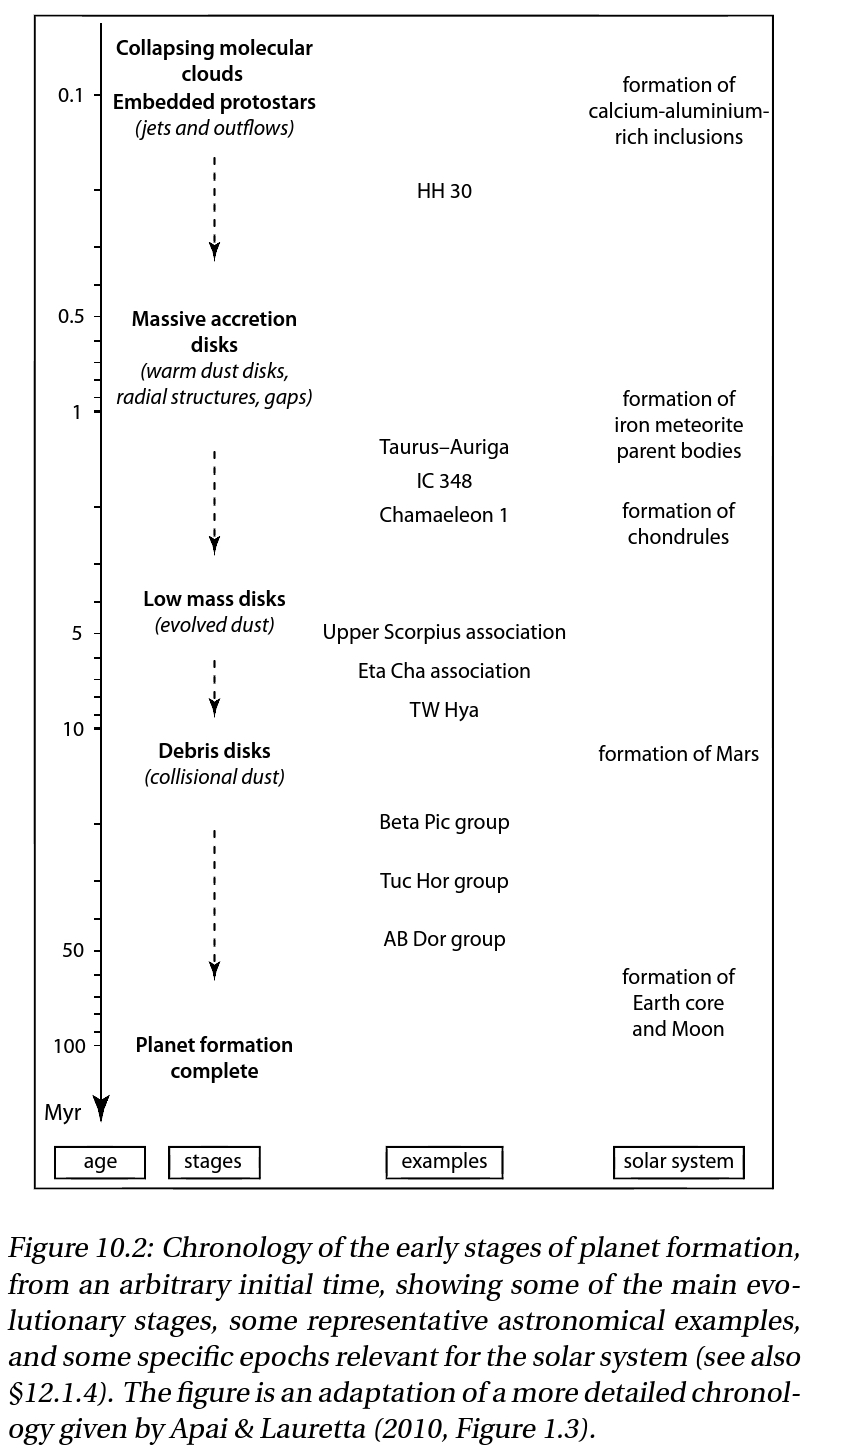
\includegraphics[trim={0cm 0cm 0 0},clip, keepaspectratio,width=0.9\textwidth]{YSOseq}\label{fig:YSOseq}\end{figure} 
\end{column}\end{columns}
\end{frame}

\begin{wordonframe}{YSO litterature}
YSO - winds, outflow and jets (HeHa: accretion interaction with B and rotation)
IR index class: Adams 87, Gail hoppe 10, Wolff 11
chemical composition: semenov 10, min 10
protostellar and protoplanetary rev: Benz 00, Dominik 07, ciesla dullemond 10, dullemond monnier 10, Youdin 10, armitage 11, beuther 14, dutrey 14, Inutsuka 14, Johansen 14, Birnstiel 16, Baruteau 16
\end{wordonframe}

\begin{wordonframe}{Cluster survey for proplyds}

\end{wordonframe}

\begin{frame}{PPD mass estimation}
Andrews williams 07, WILLIAMS cieza 11, testi 14, Andrew 15 ... ???
\end{frame}

\begin{frame}{Dust mass}
Dust emission intesity depends on temperature and optical depth ($\Sigma_{perp}\kappa$); Mie theory: particle interact with radiation at wavelength comparable to their size. At mm wavelength $\nu\approx\SI{300}{\giga\hertz}$ emission is optically thin for $\Sigma_d<\frac{1}{\kappa_{\nu}}\approx\SI{3}{\gram\per\square\cm}$: the dust mass is proportional to mm flux $M_{dust}=\frac{F_{\nu}d^2}{\kappa_{\nu}B_{\nu}(T_d)}$, d is the source's distance.
agglomeration of submicron to meter is fast (kleine 02): at least until selfgravity becomes important number density of a particle with size a that evolve through agglomeration and collision follows $N(a)\propto a^p$, $p\approx3.5$ (testi 14): total surface emitting area $\propto\int a^2N(a)\,da$ is dominated by smallest grain but total mass $\propto\int a^3N(a)\,da$ is mostly within largest
\end{frame}

\begin{wordonframe}{proplyds ages, mass, accretion rate}
accretion rate vs stellar age: hillenbrand 2005 (''Observational Constraints on Dust Disk Lifetimes: Implications for Planet Formation''); williams 12 (''Astronomical evidence for the rapid growth of mm-sized particles in proplyds); eisner 18 (''protoplanetary disk properties in orion nebula cluster'')
\end{wordonframe}

\begin{frame}{Disk viscosity and turbulence}
accretion rate for active circumstellar disk around T-tauri star: \numrange{e-9}{e-7}$\msun{}\si{\per\year}$ (Gullbring 98)
\end{frame}

\section{Disco di accrescimento: gas e polvere.}\linkdest{accretion}

\begin{frame}{Different drag regimes for different particles size}
\begin{itemize}
\item Dust (submicron-cm): coupled to gas with slow vertical-radial drift. Growth through collisions.
\item Rocks ($\approx\si{\meter}$): keplerian orbit plus aerodynamical drag
\item Planetesimal $\geq\si{\kilo\meter}$: N-body problem involving primarily gravitational forces (and strength for smaller)
\item $\approx\mearth$: coupled to disk through gravitational rather aerodynamic interactions.
\item planetary cores: around $10\mearth$ transition from quasi-hydrostatic to rapid accretion regime.
\end{itemize}
\end{frame}

\begin{frame}{Settling timescale}
\begin{block}{laminar flow}
\begin{columns}[T]\begin{column}{0.4\textwidth}
\begin{align*}
&F_D=-\frac{1}{2}C_D\pi a^2\rho v^2\\
&t_{fric}=\frac{mv}{|F_D|}\\
&t_{settle}=\frac{z}{|v_{settle}|}
\end{align*}
\end{column}\begin{column}{0.6\textwidth}
\begin{align*}
&t_{fric}(\SI{1}{\astronomicalunit};\rho=\SI{5e-10}{\gram\per\cubic\cm},\rho_d=\SI{3}{\gram\per\cubic\cm})=\SI{2.5}{\second}\\
&t_{settle}|_{z=h,a=\SI{1}{\astronomicalunit}}=\SI{2e+5}{\year} 
\end{align*}
\end{column}\end{columns}
\end{block}
\begin{block}{Turbulent flow}
\begin{columns}[T]\begin{column}{0.5\textwidth}
\begin{align*}
&t_{diffuse}=\frac{z^2}{D}\\
&t_{diffuse}(h)=t_{settle}(h): D\geq\frac{\pi\sqrt{e}}{2}\frac{\rho_mah^2\Omega_K}{\Sigma}
\end{align*}
\end{column}\begin{column}{0.5\textwidth}
\begin{align*}
&D\approx\nu=\frac{\alpha c_s^2}{\Omega_K}\\
&\alpha\geq\frac{\pi\sqrt{e}}{2}\frac{\rho_d a}{\Sigma}\\
&\alpha_{a=1\si{\micro\meter}}\geq\num{e-5},\ \alpha_{a=1\si{\milli\meter}}\geq\num{e-2}
\end{align*}
\end{column}\end{columns}
\end{block}
\end{frame}


\section{Disco primordiale e planetesimi: schemi di formazione}\linkdest{sec:formationschemes}

\subsection{Condizione di instabilit\'a}

\begin{frame}{Schema a l\'a Safronov/Cameron}
\begin{block}{Disco minimale}
Ogni pianeta si \'e formato in un anello del disco iniziale la cui massa \'e quella che ristabilisce la proporzione fra le abbondanze dei varii elementi solari (o galattiche): $M_{disk}(\SI{50}{\astronomicalunit})\approx0.04\msun{}$.
\end{block}
\begin{block}{Schema a l\'a Safronov}
Sedimentazione della componente polverosa in disco di pi\'u piccola massa. Instabilit\'a della polvere. $M_{disk}\approx\numrange{e-1}{e-2}\msun{}$.
Accrezione blocchi solidi ($\approx\SI{1}{\meter}$).
\end{block}
\begin{block}{Modello alla Cameron}
Instabilit\'a gravitazionale dell'intero disco. $M_{disk}\approx\msun{}$.
\end{block}
\end{frame}

\begin{wordonframe}{Schema Safronov/Cameron}
\begin{block}{Densit\'a superficiale}
\begin{align*}
&\sigma(r)\approx(\frac{r}{\SI{8e13}{cm}})\expy{-\frac{3}{2}}\si{\gram\per\cubic\cm}\\
&\int^{\SI{50}{\astronomicalunit}}\sigma(r)\,dr=0.04\msun{}
\end{align*}
\end{block}
Schema a l\'a Safronov: sedimentazione polvere verso il piano equatoriale.
Il criterio di Jeans non \'e applicabile: potenziale gravitazionale non \'e costante. (Forze mareali)
\end{wordonframe}

\begin{frame}{Struttura verticale del disco}
\begin{block}{Equilibrio idrostatico}
\begin{equation*}
\TDy{z}{P}=-\rho g_z=-\rho\frac{GM}{a^2}\frac{z}{a}\ \Rightarrow\ \rho(z)=\rho(0)\exp{-\frac{GMm}{a^3kT}z^2}
\end{equation*}
\end{block}
\begin{block}{Spessore effettivo}
\begin{columns}[T]
\begin{column}{0.5\textwidth}
\begin{align*}
&H=\frac{1}{\rho(0)}\int\rho(z)\,dz\\
&\frac{H}{a}\approx\sqrt{\frac{akT}{GMm}}
\end{align*}
\end{column}
\begin{column}{0.5\textwidth}
Per $a_J$, $T\approx\SI{100}{\kelvin}$, $H_2$: $\frac{H}{a}\approx0.1$.
Equipartizione energia gas/polvere:
\begin{equation*}
(\frac{H}{a})_{pol}=(\frac{H}{a})_{gas}\sqrt{\frac{m_{gas}}{m_{pol}}}
\end{equation*}
\end{column}
\end{columns}
\end{block}
\begin{block}{Equilibrio radiativo con la stella}
\begin{equation*}
T\propto a\expy{-\frac{1}{2}}\ \Rightarrow\ \frac{H}{a}\propto a \expy{\frac{1}{4}}\ (\propto a \expy{\frac{1}{8}})
\end{equation*}
\end{block}
\begin{columns}[T]
\begin{column}{0.4\textwidth}
\begin{block}{Instabilit\'a della polvere}
\begin{equation*}
\rho_{pol}^{cr}\approx\frac{\msun{}}{a^3}=\rho_{gas}X_{pol}\frac{H_{gas}}{H_{pol}}
\end{equation*}
\end{block}
\end{column}
\begin{column}{0.6\textwidth}
\begin{block}{Ruolo turbolenza}
\begin{itemize}
\item Impedisce sedimentazione disco di polvere
\item Crea addensamenti potentialmente instabili (Johansen 2007)
\end{itemize}
\end{block}
\end{column}
\end{columns}
\end{frame}

\begin{wordonframe}{Struttura verticale del disco}
Assumendo che $P=\frac{kT}{m}\rho$.
Equilibrio termico con la stella: $T^4R^2=\const{}$. Energy flux: $T_e^P=T_e^*\sqrt{\frac{R_*}{r_{*P}}}$.
$m_{pol}\approx\num{e12}m_{gas}$.
\end{wordonframe}

\subsection{Evoluzione oltre planetesimi: how do planetesimal growth to form embryos?}

\begin{wordonframe}{planetesimal-gas residual interactions}
Residual aerodynamics interactions damps e,i while density fluctuations produced by turbulence exert fluctuating gravitational force that excite eccentricity (laughlin steinacker adams 04; nelson 05; okuzumi ormel 13). Limited planetesimal-gas interactions until badies larger than \SI{e3}{\kilo\meter}.
\end{wordonframe}

\begin{frame}{Collisional accretion}
\begin{columns}[T]\begin{column}{0.5\textwidth}
sum of radii $R_s>R_c$ there will be a collision: conservation of E and L give greatest value to have collision
\[b^2=R_s^2+\frac{4GmR_s}{\sigma^2}\]
\[b^2=R_s^2(1+\frac{v_{esc}^2}{\sigma^2}\]
e la sezione d'urto per collisioni \'e $\Gamma=\pi b^2$.
\end{column}\begin{column}{0.5\textwidth}
\begin{figure}[!ht]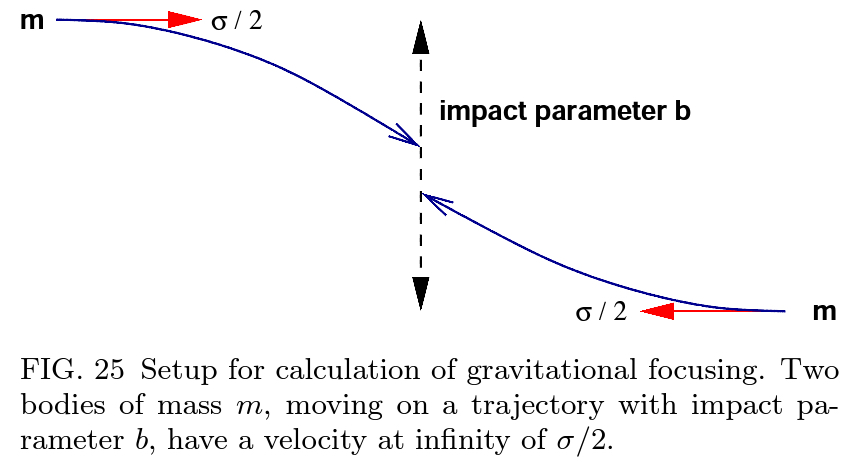
\includegraphics[trim={0cm 0cm 0 0},clip, keepaspectratio,width=0.5\textwidth]{impactparam}\label{fig:impactparam}\end{figure}
\end{column}\end{columns}
\end{frame}

\begin{frame}{Outcomes of collisions: accretion, shattering, dispersal}
\begin{columns}[T]\begin{column}{0.5\textwidth}

\end{column}\begin{column}{0.5\textwidth}

\end{column}\end{columns}
\end{frame}

\subsection{Evoluzione planetesimi}

\begin{frame}{Dinamica dei planetesimi}
\begin{block}{Two body relaxation}
\begin{columns}[T]\begin{column}{0.4\textwidth}
\begin{align*}
&\TtwoDy{t}{\vec{x}_i}=-GM_*\frac{\vec{x}_i}{|x_i^3|}+\sum_{i\neq j}Gm_j\frac{\vec{x}_i-\vec{x}_j}{|\vec{x}_i-\vec{x}_j|^3}\\
&+\vec{F}_{gas}+\vec{F}_{col}\\
&t_{rel}=\frac{\sigma^2}{\TDy{t}{\sigma^2}}\approx\frac{1}{n\pi r_g^2\sigma\ln{\Lambda}}\\
&=\frac{\sigma^3}{n\pi G^2m^2\ln{\Lambda}}
\end{align*}
\end{column}\begin{column}{0.6\textwidth}
deviation from local circular orbit, random velocity, $v=\sqrt{i^2+e^2}v_K$; timescale for 2b relaxation for equal-m many-body system: (n)umber density, $r_g=\frac{Gm}{\sigma^2}$ gravitational radius, $n\pi r_g^2\sigma$ number of close encounter with $\Delta\theta>\pi/2$, $\ln{\Lambda}$ accounts for distant encounters
\end{column}\end{columns}
\end{block}

\end{frame}

\begin{frame}{}

\end{frame}

\subsection{Evoluzione collisionale proto-pianeti}

\begin{frame}{Accrescimento dei planetesimi: collisioni.}
\begin{itemize}
\item $r_{pl}<b<\frac{Gm_{pl}}{v_r^2}=b_0$: incontro ravvicinato ($|U_{max}|>E_{kin}^{\infty}$).
\item $b>(\frac{m_{pl}}{3\msun{}})\expy{\frac{1}{3}}a=d_{Hill}$: passaggio a grande distanza.
\item $b_0<b<d_{Hill}$: deflessioni di direzione e verso casuali.
\end{itemize}
\begin{block}{Scattering $b>r_{pl}$: variazione velocit\'a relativa}
\begin{equation*}
\delta v_r=\underbrace{\frac{Gm_{pl}}{b^2}}_{\exv{a}}\underbrace{\frac{2b}{v_r}}_{\exv{\tau_{int}}}=\frac{2Gm_{pl}}{bv_r}
\end{equation*}
\end{block}
\begin{equation*}
b_0<b<d_{Hill}:\quad [\TDy{t}{v_r^2}]_{enc}=\int_{r_{pl}}^d2\pi bv_r\frac{\sigma n}{m_{pl}v_r}(\frac{2Gm_{pl}}{bv_r})^2\,db
\end{equation*}
\begin{block}{Urti anelastici: impatti}
\begin{equation*}
[\TDy{t}{v_r^2}]_{imp}=\pi r_{pl}^2(\frac{\sigma n}{m_{pl}v_r})v_r(-v_r)
\end{equation*}
\end{block}
\end{frame}

\begin{wordonframe}{evoluzione collisionale pp}
Dato semiasse a e eccentricit\'a media e i corpi si incontrano se compresi in fascia di larghezza ae,$v_r\approx ena$.
Densit\'a numerica planetesimi: $\rho_{pl}\approx\frac{\sigma n}{m_{pl}v_r}$.
Variazione velocit\'a relativa media $\exv{\delta v_r}$ 
Diffusione nello spazio delle velocit\'a: aumento $\exv{e}\approx\exv{i}$ (random walk), a meno di risonanze.
\begin{itemize}
\item $r_{pl}<b<\frac{Gm_{pl}}{v_r^2}=b_0$: incontro ravvicinato ($|U_{max}|>E_{kin}^{\infty}$).
\item $b>(\frac{m_{pl}}{3\msun{}})\expy{\frac{1}{3}}a=d_{Hill}$: passaggio a grande distanza.
\item $b_0<b<d_{Hill}$: deflessioni di direzione e verso casuali, $\exv{\delta v_r}=0$,
\begin{equation*}
[\TDy{t}{v_r^2}]_{enc}=\int_{r_{pl}}^d2\pi bv_r\frac{\sigma n}{m_{pl}v_r}(\frac{2Gm_{pl}}{bv_r})^2\,db
\end{equation*}
\end{itemize}
Lobo di Hill: nel problema a 3 corpi \'e la regione in cui l'influenza del pianeta prevale su quella solare. Zona di Giove:
\begin{equation*}
\frac{\rho_{pl}}{3\rho_{\odot}}\approx\frac{1}{4}\ \Rightarrow\ d=(\frac{\rho_{pl}}{3\rho_{\odot}})\expy{\frac{1}{3}}r_{pl}\frac{a}{\rsun{}}\approx600r_{pl}
\end{equation*}
\end{wordonframe}

\begin{frame}{Evoluzione della velocit\'a relativa}
\begin{block}{Il sistema evolve verso stato stazionario}
\begin{align*}
&\TDy{t}{v_r}=[\TDy{t}{v_r}]_{enc}+_?[\TDy{t}{v_r}]_{imp}=\pi\frac{\sigma n}{m_{pl}}r_{pl}v_r[(\frac{v_e}{v_r})^4\ln{(\frac{d}{r_{pl}})}-1]\\
&\tau\approx\frac{m_{pl}}{\pi r_{pl}^2\sigma n}\approx\SI{e6}{\year}
\end{align*}
Il sistema evolve in tempo $\tau$ verso stato stazionario con $v_r\approx v_e$.
\end{block}
\begin{block}{Runaway growth}
Il pianeta pi\'u massiccio cresce pi\'u velocemente: contributo gravitazionale alla sezione d'urto
\begin{equation*}
\sigma_{imp}=\pi b_i\approx\pi r_{pl}^2(1+\frac{v_e^2}{v_{\infty}^2})
\end{equation*}
Il frammento pi\'u grosso determina la dinamica dell'intera zona: $v_r^2=\frac{Gm_1}{\theta r_1}$.
\end{block}

\end{frame}

\begin{wordonframe}{Evoluzione $v_r$}

$\tau$ piccolo rispetto tempi crescita embrioni planetari.

$\theta$ ($\approx1-100$) parametro di Safronov, $m_1$, $r_1$ massa e raggio del maggior embrione.

($\sigma_i\propto r_{pl}^4$ for small $v_{\infty}$.

\end{wordonframe}

\subsection{Formazione pianeti giganti e corpi minori}

\begin{frame}{Formazione di corpi minori: evoluzione collisionale a grande $v_r$}
\begin{block}{Collisioni ad alta velocit\'a relativa}
La velocit\'a relativa aumenta con la massa dell'embrione planetario: $v_r^2=\frac{Gm_1}{\theta r_1}$.

Aumentano $\exv{e}$ e $\exv{i}$: fascia di cattura pi\'u ampia.
\end{block}
\begin{block}{Espulsione di materia nelle fasi finali di accumulazione}
\begin{equation*}
v_{es}=(\sqrt{2}-1)\sqrt{\frac{G\msun{}}{a}}
\end{equation*}
Perturbazioni di orbite esterne possono determinare deflessione verso l'interno: main belt, late heavy bombardament.
\end{block}

\end{frame}

\begin{wordonframe}{formazione corpi minori}
$v_{es}$ orbita circolare: $\theta_{es}=\frac{1}{3-2\sqrt{2}}\sqrt{\frac{G\msun{}}{a}}$; $\theta_{es}\approx100$ per pianeti esterni in fase finale di formazione.

Espulsione di grande quantit\'a di materia nelle fasi finali di accumulazione
\end{wordonframe}

\begin{frame}{Cattura di gas}
\begin{itemize}
\item Massa embrione planetario
\item Temperatura locale
\item Rapidit\'a di formazione del proto-pianeta
\end{itemize}
Il modello a l\'a Safronov spiega la differenza di composizione dei pianeti.
\end{frame}

\begin{wordonframe}{Capacit\'a degli embrioni planetari di catturare gas}
Pi\'u il gas \'e freddo pi\'u \'e probabile la cattura.
\end{wordonframe}

\subsection{Leggi di scala nel modello a l\'a Safronov}

\begin{frame}{Legge di Titus-Bode (Armellini): pianeti, satelliti maggiori.}
\begin{equation*}
a(\si{\astronomicalunit})=B+C 2^n,\quad B\approx0.4,\ C\approx0.3
\end{equation*}
\begin{itemize}
\item Pianeti catturano tutto il materiale in una fascia attorno all'orbita.
\item Le zone di cattura sono continue e non si sovrappongono.
\end{itemize}
\begin{align*}
&\Delta a_{tot}\approx[\exv{e}+(\frac{m_{pl}}{\msun{}})^{\xi}]\approx\const{}a\\
&a_{n+1}=a_n+\frac{\Delta a_n}{2}+\frac{\Delta a_{n+1}}{2}\ \Rightarrow\ \frac{a_n}{a_{n+1}}=\const
\end{align*}
Le deviazioni dall'andamento medio favoriscono l'isolamento dei pianeti.
\end{frame}

\begin{wordonframe}{Formulazione alla armellini di TB.}
I semiassi dei pianeti (satelliti maggiori) costituiscono una serie geometrica approssimata.

Cattura geometrica, $\exv{e}$ eccentricit\'a media corpi piccoli: $\Delta a\approx\exv{e}a$.

Cattura gravitazionale: $\Delta a\approx(\frac{m_{pl}}{\msun{}})\expy{\xi}a$, $\xi\approx\frac{1}{3}$ (lobo di Hill), $\xi\approx\frac{1}{4}$ (Dole 1960).

Ipotesi semplificativa: $\Delta a_{tot}=\Delta a _{geo}+\Delta a_{gra}$.
\begin{align*}
&\Delta a_{tot}\approx[\exv{e}+(\frac{m_{pl}}{\msun{}})^{\xi}]\approx\const{}a\\
&a_{n+1}=a_n+\frac{\Delta a_n}{2}+\frac{\Delta a_{n+1}}{2}\ \Rightarrow\ \frac{a_n}{a_{n+1}}=\const
\end{align*}
Dove $\exv{e}$ varia lentamente con a, $m_{pl}$ non troppo grande, $\xi$ piccolo.

Tenendo conto delle risonanze (Wisdom 80/Lissauer 95): $\Delta a\approx(\frac{m_{pl}}{\msun{}})\expy{\frac{2}{7}}a$.
\end{wordonframe}

\begin{frame}{Scaling law}
Condensazione di tutto il materiale: $m_{pl}=2\pi a\sigma\Delta a$.

\begin{equation*}
\Delta a=(\frac{m_{pl}}{\msun})\expy{\gamma}a\ \Rightarrow\ m_{pl}\propto a\expy{\frac{2}{1-\gamma}}\sigma\expy{\frac{1}{1-\gamma}}\msun{}\expy{-\frac{\gamma}{1-\gamma}}
\end{equation*}

Dischi massicci producono meno pianeti ma pi\'u grossi:
\begin{equation*}
N_p=\frac{M_{disk}}{m_{pl}}\propto(\frac{M_{disk}}{\msun{}})\expy{-\frac{\gamma}{1-\gamma}}
\end{equation*}
$\gamma=\frac{2}{7}$, $\gamma=\frac{1}{4}$, $\gamma=\frac{1}{3}$ (Hill).

\end{frame}

\begin{wordonframe}{Scaling law}
\begin{equation*}
M_{disk}=a^2\sigma\ \Rightarrow\ m_{pl}\propto M_{disk}\expy{\frac{1}{1-\gamma}}M_*\expy{-\frac{\gamma}{1-\gamma}}=M_{disk}(\frac{M_{disk}}{M_*})\expy{\frac{\gamma}{1-\gamma}}
\end{equation*}
\end{wordonframe}

\section{Migrazione planetaria}\linkdest{sec:migration}

\begin{frame}{Problemi nei modelli di formazione}
\begin{itemize}
\item Assenza di asteroidi oltre \SI{3.3}{\astronomicalunit}.
\item Scarsezza di oggetti nella regione di Kuiper interna a Plutone.
\item Nei sistemi extra-solari sono osservati pianeti pi\'u massicci di Giove a distanze minori (Effetti di selezione)
\end{itemize}
I dischi circumstellari tipicamente osservati hanno masse caratteristiche dei modelli a l\'a Safronov.
\end{frame}

\begin{frame}{Processi che determinano migrazione planetaria}

\begin{itemize}
\item Interazione pianeti in formazione disco (Goldreich, Tremaine 1980).
\item Scattering pianeta-corpi minori sopravvissuti alla fase di formazione.
\item Instabilit\'a dinamica causata da presenza di 2 pianeti massicci in orbite vicine (Jumping Jupiters): osservati in sistemi extra-solari.
\end{itemize}

\end{frame}

\begin{frame}{Interazione disco-pianeta}
\begin{block}{Risonanze}
\begin{itemize}
\item Corotazione: frequenza orbitale del disco e del pianeta coincidono
\item Risonanze di Lindblad: migrazione verso l'interno (tipo I)
\end{itemize}
\end{block}

\begin{block}{Rallentamento migrazione}
$\tau_{mig}\propto\frac{1}{m_{pl}}$: caduta troppo rapida sulla stella
\begin{itemize}
\item Azione efficace risonanze di Lindblad impedito da formazione gap attorno al pianeta massiccio
\item per pianeti massicci si ha svuotamento anello attorno orbita planetaria
\item turbolenza su larga scala
\item campo magnetico della stella
\item interazioni mareali/scambi di massa stella/pianeta
\end{itemize}
\end{block}
\end{frame}

\begin{wordonframe}{interazione disco-pianeta: risonanze}
Vedi interazione satellite-anelli.

Orbita eccentrica: corotazione con diverse parti del disco.

Le risonanze di Lindblad interne tendono a far migrare il pianeta verso l'esterno e viceversa. L'effetto della risonanza esterna prevale regolarmente.

Il momento angolare scambiato ad ogni risonanza \'e proporzionale a $m_{pl}^2$.

Disco massiccio e pianeta massiccio determinano migrazione veloce. Il modello spiega la scarsezza di brown dwarf. In $\tau\approx\SI{e5}{\year}$ un pianeta di qualche massa terrestre spiraleggia sulla stella.

Fascia vuota attorno all'orbita: diffusione non riesce a mantenere uniforme la densit\'a.
Turbolenza introduce termine stocastiuco nella migrazione.

\end{wordonframe}

\subsection{Jumping Jupiters}

\begin{frame}{Stabilit\'a dinamica}
\begin{block}{Stabilit\'a dinamica sistema a 3 corpi}
\begin{equation*}
\Delta=a_2-a_1>2\sqrt{3}R_{H12}\approx2.4a_1(\mu_1+\mu_2)\expy{\frac{1}{3}},\ \mu_i=\frac{\mu_i}{M_*}
\end{equation*}
Per Sole-Giove-Saturno: $a_S-a_J=\SI{4.2}{\astronomicalunit}>\SI{1.4}{\astronomicalunit}$.
\end{block}
\begin{block}{Stabilit\'a dinamica sistema a molti corpi}
Simulazioni numeriche (Marzari, Weidenschilling 2002): 3 pianeti con $m_i\approx m_J$, $a_i=a_{i-1}+kR_{Hi,i-1}$.

Il risultato pi\'u probabile \'e l'espulzione di un pianeta e l'immissione di un altro su orbita interna eccentrica: per i sistemi pi\'u stretti sono spiegati dalla migrazione.
\end{block}
\end{frame}

\begin{wordonframe}{Stabilit\'a dinamica orbite}
Lobo di Hill: $R_{H12}=(\frac{m_1+m_2}{M_*})\expy{\frac{1}{3}}\frac{a_1+a_2}{2}$.

Limite alla migrazione dalla conservazione dell'energia:
\begin{align*}
&E_i=-\frac{GM_*}{2}(\frac{m_1}{a_1}+\frac{m_2}{a_2}+\frac{m_3}{a_3})\approx\const{}\\
&E_f=-\frac{GM_*}{2}(\frac{m_3}{a_{3f}}+\frac{m_2}{a_{2f}})\approx-\frac{GM_*m_3}{2a_{3f}}\\
&\Rightarrow a_{3f}\approx\frac{1}{\frac{1}{a_1}+\frac{1}{a_2}+\frac{1}{a_3}}>\frac{a_1}{3}
\end{align*}
Sistemi con pianeti relativamente vicini e orbite eccentriche hanno spesso pianeta massiccio esterno.
\end{wordonframe}

\section{Formazione del sistema solare}\linkdest{sec:nizza}

\subsection{Dating}

\begin{wordonframe}{Refs}
''THE Hf-WISOTOPIC SYSTEM AND THE ORIGIN OF THE EARTH AND MOON'' Jacobsen 05
''A short timescale for terrestrial planet formation from Hf-W chronometry of meteorites''
\end{wordonframe}

\begin{frame}{Modello di Nizza}

Scattering planetesimi causa la migrazione dei pianeti giganti.

\begin{block}{Regione formazione pianeti giganti}
\begin{itemize}
\item Giove \SI{5.45}{\astronomicalunit} (\SI{5.2}{\astronomicalunit})
\item Saturno \SI{8.5}{\astronomicalunit} (\SI{1}{\astronomicalunit})
\item Urano e Nettuno \SI{11}{\astronomicalunit} e \SI{17}{\astronomicalunit}
\end{itemize}
\end{block}
\begin{block}{Late heavy bombardament}
Quando Saturno attraversa la risonanza $2:1$ con Giove si ha una fase di intensa eccitazione dinamica: crateri lunari datano a \SI{3.8}{\giga\year} fa. (cattura troiani)
\end{block}
\end{frame}
            